%% ============================================================
%%  Airbnb New User Booking Analytics – Beamer Presentation
%%  Compile with: pdflatex presentation.tex  (run twice)
%% ============================================================
\documentclass[aspectratio=169]{beamer}

% ── Theme ─────────────────────────────────────────────────────────────────────
\usetheme{Madrid}
\usecolortheme{default}

% ── Airbnb brand colours ──────────────────────────────────────────────────────
\definecolor{AirRed}{HTML}{FF5A5F}
\definecolor{AirTeal}{HTML}{00A699}
\definecolor{AirDark}{HTML}{484848}
\definecolor{AirLight}{HTML}{F7F7F7}

\setbeamercolor{palette primary}{bg=AirRed, fg=white}
\setbeamercolor{palette secondary}{bg=AirDark, fg=white}
\setbeamercolor{palette tertiary}{bg=AirTeal, fg=white}
\setbeamercolor{palette quaternary}{bg=AirDark, fg=white}
\setbeamercolor{structure}{fg=AirRed}
\setbeamercolor{frametitle}{bg=AirRed, fg=white}
\setbeamercolor{title}{bg=AirRed, fg=white}
\setbeamercolor{block title}{bg=AirTeal, fg=white}
\setbeamercolor{block body}{bg=AirLight, fg=AirDark}
\setbeamercolor{alerted text}{fg=AirRed}

% ── Packages ──────────────────────────────────────────────────────────────────
\usepackage[utf8]{inputenc}
\usepackage[T1]{fontenc}
\usepackage{lmodern}
\usepackage{booktabs}
\usepackage{graphicx}
\usepackage{xcolor}
\usepackage{hyperref}
\usepackage{tikz}
\usepackage{pgfplots}
\pgfplotsset{compat=1.18}

% ── Metadata ──────────────────────────────────────────────────────────────────
\title[Airbnb Analytics Dashboard]{Airbnb New User Booking Analytics\\[4pt]
       \large An Interactive Multi-Page Dashboard}
\author{Taron Khachatryan}
\institute{Data Visualisation — Final Project}
\date{May 2026}

% ── Helper: coloured badge ────────────────────────────────────────────────────
\newcommand{\badge}[2]{%
  \tikz[baseline=(x.base)]\node[fill=#1,text=white,rounded corners=2pt,
        inner xsep=4pt,inner ysep=2pt,font=\small\bfseries](x){#2};%
}

% ==============================================================
\begin{document}
% ==============================================================

% ── Title frame ───────────────────────────────────────────────────────────────
\begin{frame}
  \titlepage
\end{frame}

% ── Outline ───────────────────────────────────────────────────────────────────
\begin{frame}{Outline}
  \tableofcontents
\end{frame}

% ══════════════════════════════════════════════════════════════
\section{Dataset Introduction}
% ══════════════════════════════════════════════════════════════
\begin{frame}{Dataset Introduction}
  \begin{columns}[T]
    \begin{column}{0.55\textwidth}
      \textbf{Source:} Kaggle --- \emph{Airbnb New User Bookings}\\[6pt]
      \begin{block}{Training Set}
        \begin{itemize}
          \item \textbf{213,451} user records
          \item Date range: 2010 -- 2014
          \item 16 raw feature columns
        \end{itemize}
      \end{block}
      \vspace{6pt}
      \begin{block}{Test Set}
        \begin{itemize}
          \item 62,096 records (no label)
        \end{itemize}
      \end{block}
    \end{column}
    \begin{column}{0.42\textwidth}
      \textbf{Key features used:}\\[4pt]
      \begin{tabular}{ll}
        \toprule
        Feature & Type \\
        \midrule
        \texttt{gender}          & Categorical \\
        \texttt{age}             & Numeric \\
        \texttt{signup\_method}  & Categorical \\
        \texttt{first\_device}   & Categorical \\
        \texttt{language}        & Categorical \\
        \texttt{date\_account\_created} & Date \\
        \texttt{country\_destination}   & \alert{Target} \\
        \bottomrule
      \end{tabular}
    \end{column}
  \end{columns}
\end{frame}

% ══════════════════════════════════════════════════════════════
\section{Problem Statement}
% ══════════════════════════════════════════════════════════════
\begin{frame}{Problem Statement}
  \begin{block}{Core Question}
    \centering
    \large\textit{``Where will a new Airbnb user make their \textbf{first} booking?''}
  \end{block}
  \vspace{10pt}
  \begin{columns}[T]
    \begin{column}{0.48\textwidth}
      \textbf{Target classes (12):}
      \begin{itemize}
        \item \alert{\texttt{NDF}} --- No booking made
        \item \texttt{US} --- United States
        \item \texttt{other} --- Unlisted country
        \item \texttt{FR, IT, GB, ES, CA,}\\
              \texttt{DE, NL, AU, PT}
      \end{itemize}
    \end{column}
    \begin{column}{0.48\textwidth}
      \textbf{Analytical challenges:}
      \begin{itemize}
        \item Severe class imbalance\\(\texttt{NDF} $\approx$\,58\,\%)
        \item Large proportion of missing ages ($\approx$\,43\,\%)
        \item Outlier ages removed ($<15$ or $\geq100$)
        \item Sparse long-tail destinations
      \end{itemize}
    \end{column}
  \end{columns}
\end{frame}

% ══════════════════════════════════════════════════════════════
\section{Key Insights}
% ══════════════════════════════════════════════════════════════

% ── Insight 1: Conversion funnel ─────────────────────────────
\begin{frame}{Key Insight 1 — Conversion Funnel}
  \begin{columns}[T]
    \begin{column}{0.5\textwidth}
      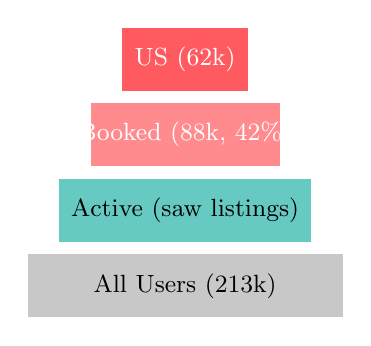
\begin{tikzpicture}[scale=0.80]
        % Simple funnel bars
        \fill[AirDark!30] (0,0) rectangle (5, 1.0) node[midway,black]{\small All Users (213k)};
        \fill[AirTeal!60] (0.5,1.2) rectangle (4.5, 2.2) node[midway,black]{\small Active (saw listings)};
        \fill[AirRed!70]  (1.0,2.4) rectangle (4.0, 3.4) node[midway,white]{\small Booked (88k, 42\%)};
        \fill[AirRed]     (1.5,3.6) rectangle (3.5, 4.6) node[midway,white]{\small US (62k)};
      \end{tikzpicture}
    \end{column}
    \begin{column}{0.47\textwidth}
      \begin{itemize}
        \item \textbf{58\%} of users never book (\texttt{NDF})
        \item Among bookers, \textbf{70\%} choose the US
        \item Next destinations: \texttt{other}, \texttt{FR}, \texttt{IT}
        \item Strong home-market bias typical of\\
              early-stage marketplace growth
      \end{itemize}
      \vspace{8pt}
      \badge{AirRed}{Takeaway} US-first product strategy validated.
    \end{column}
  \end{columns}
\end{frame}

% ── Insight 2: Demographics ───────────────────────────────────
\begin{frame}{Key Insight 2 — User Demographics}
  \begin{columns}[T]
    \begin{column}{0.48\textwidth}
      \begin{block}{Age Profile}
        \begin{itemize}
          \item Median age $\approx$ \textbf{34 years}
          \item Peak cohort: \textbf{25--35} years
          \item Very few users over 60\\
                (older users less represented)
        \end{itemize}
      \end{block}
      \vspace{6pt}
      \begin{block}{Gender}
        \begin{itemize}
          \item Near 50/50 split (after removing \texttt{-unknown-})
          \item Slight female majority in bookers
        \end{itemize}
      \end{block}
    \end{column}
    \begin{column}{0.48\textwidth}
      \begin{block}{Device \& Signup}
        \begin{itemize}
          \item \textbf{Mac / iPhone} dominate ($>$60\%)
          \item Reflects affluent, tech-forward user base
          \item \textbf{Basic} signup method most common
          \item Facebook OAuth accounts grow rapidly post-2012
        \end{itemize}
      \end{block}
      \vspace{6pt}
      \badge{AirTeal}{Takeaway} Target marketing at 25--35,\\
      Mac-using urban professionals.
    \end{column}
  \end{columns}
\end{frame}

% ── Insight 3: Growth trends ──────────────────────────────────
\begin{frame}{Key Insight 3 — Platform Growth Trends}
  \begin{columns}[T]
    \begin{column}{0.55\textwidth}
      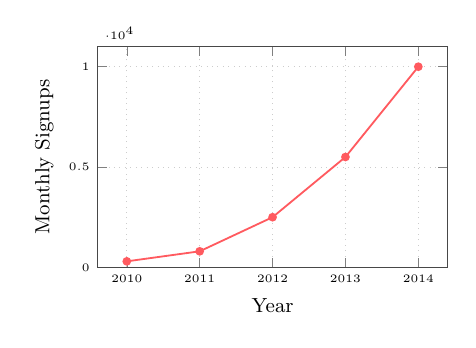
\begin{tikzpicture}[scale=0.82]
        \begin{axis}[
          xlabel={Year}, ylabel={Monthly Signups},
          xtick={2010,2011,2012,2013,2014},
          xticklabels={2010,2011,2012,2013,2014},
          ymin=0, ymax=11000,
          width=7cm, height=5cm,
          grid=both, grid style={dotted,gray!40},
          tick label style={font=\tiny},
          label style={font=\small},
          axis line style={AirDark},
        ]
          \addplot[AirRed, thick, mark=*, mark size=1.5pt] coordinates {
            (2010, 300)
            (2011, 800)
            (2012, 2500)
            (2013, 5500)
            (2014, 10000)
          };
        \end{axis}
      \end{tikzpicture}
    \end{column}
    \begin{column}{0.42\textwidth}
      \begin{itemize}
        \item Approximately \textbf{33$\times$} growth from 2010 to 2014
        \item Consistent \textbf{summer peaks} (Jun--Aug)\\
              year-over-year
        \item 2013--2014: inflection point driven by\\
              mobile app adoption
        \item Growth slows in H2 2014 in training data\\
              (data collection artefact)
      \end{itemize}
      \vspace{6pt}
      \badge{AirDark}{Takeaway} Seasonal campaigns in summer\\
      maximise acquisition ROI.
    \end{column}
  \end{columns}
\end{frame}

% ══════════════════════════════════════════════════════════════
\section{Dashboard Design}
% ══════════════════════════════════════════════════════════════
\begin{frame}{Dashboard Design Choices}
  \begin{columns}[T]
    \begin{column}{0.48\textwidth}
      \textbf{Architecture:}\\[4pt]
      \begin{tabular}{ll}
        \toprule
        File & Purpose \\
        \midrule
        \texttt{app.py}           & Entry point, navbar \\
        \texttt{pages/overview.py}    & KPIs, static charts \\
        \texttt{pages/demographics.py}& Interactive filters \\
        \texttt{pages/trends.py}      & Time-series controls \\
        \texttt{utils/data.py}        & Shared preprocessing \\
        \bottomrule
      \end{tabular}
    \end{column}
    \begin{column}{0.48\textwidth}
      \textbf{Design decisions:}
      \begin{itemize}
        \item Airbnb brand palette\\
              {\color{AirRed}\rule{12pt}{8pt}} \texttt{\#FF5A5F} \;
              {\color{AirTeal}\rule{12pt}{8pt}} \texttt{\#00A699}
        \item Dash Bootstrap (responsive grid)
        \item \texttt{use\_pages=True} --- clean URL routing
        \item Callbacks scoped \emph{inside} each page file
        \item Filters reset independently per page
        \item KPI cards at top for immediate context
        \item Chart-first layout: most important\\
              visualisation full-width
      \end{itemize}
    \end{column}
  \end{columns}
\end{frame}

% ══════════════════════════════════════════════════════════════
\section{Live Demo}
% ══════════════════════════════════════════════════════════════
\begin{frame}{Live Dashboard Demo}
  \begin{center}
    \Large\textbf{Deployed on Render}\\[10pt]
    \large\texttt{\href{https://airbnb-dashboard.onrender.com}{https://airbnb-dashboard.onrender.com}}\\[16pt]
    \normalsize
    \begin{tabular}{lp{8cm}}
      \badge{AirRed}{Page 1}   & \textbf{Overview} — KPI cards, destination bar chart, device pie, monthly growth line \\[6pt]
      \badge{AirTeal}{Page 2}  & \textbf{Demographics} — interactive age/gender/year filters controlling 4 live charts \\[6pt]
      \badge{AirDark}{Page 3}  & \textbf{Trends} — year selector, breakdown dropdown, destination search, country-age box \\
    \end{tabular}
  \end{center}
\end{frame}

% ══════════════════════════════════════════════════════════════
\section{Conclusions}
% ══════════════════════════════════════════════════════════════
\begin{frame}{Key Conclusions \& Findings}
  \begin{block}{Business Implications}
    \begin{enumerate}
      \item \textbf{Reduce NDF rate} — More than half of registered users never book;
            targeted email / push campaigns during the first 7 days should convert
            fence-sitters.
      \item \textbf{US-first, then Europe} — Localisation and pricing for FR, IT, GB
            represent the highest-value international opportunity.
      \item \textbf{Mobile-first design} — Mac \& iPhone dominate; iOS-native features
            have disproportionate impact on the core audience.
      \item \textbf{Seasonal marketing} — Summer surges are consistent; budget summer
            acquisition campaigns accordingly.
      \item \textbf{Young-adult focus} — The 25--35 cohort both signs up and books at
            the highest rate; retention in this group has compound long-term value.
    \end{enumerate}
  \end{block}
\end{frame}

% ── Q&A ───────────────────────────────────────────────────────────────────────
\begin{frame}
  \begin{center}
    \vspace{20pt}
    {\Huge\color{AirRed}\textbf{Thank You}}\\[16pt]
    {\large Questions \& Discussion}\\[20pt]
    \hrule\vspace{10pt}
    \small
    Dashboard source: \texttt{github.com/[your-repo]}\\
    Live URL: \texttt{https://airbnb-dashboard.onrender.com}\\
    Contact: \texttt{[your-email]}
  \end{center}
\end{frame}

\end{document}
